\documentclass[markcolor=black,spinewidth=2.5mm,coverwidth=5.5in,coverheight=8.75in,flapwidth=2.5in]{bookcover}

\usepackage[utf8]{inputenc}
\usepackage[T1]{fontenc}
\usepackage[english]{babel}
\usepackage{url}
\usepackage{contour}
\usepackage{lipsum}
\contourlength{1pt}

\begin{document}

\begin{bookcover}

\bookcovercomponent{color}{bg whole}{black}

\bookcovercomponent{picture}{whole without flaps}{output.png}

% Remark
\bookcovercomponent{center}{above front}{
    \color{red}\textsc{The Illustrated Geek} dust jacket}

% Text on the spine
\bookcovercomponent{center}{spine}{
    \rotatebox[origin=c]{90}{\footnotesize\bfseries 
        \color{white}\contour{black}{The Illustrated Geek --- Mel McCalla}}}

\bookcovercomponent{normal}{front}{
	\vspace{30.5mm}
	\centering
	{\color{white}\contour{black}{\huge\bfseries The Illustrated Geek}\\[13mm]}
	{\color{white}\contour{black}{\large\bfseries Mel McCalla}\\[10mm]}
}

\bookcovercomponent{normal}{front flap}{
	\centering
	\vspace{1in}
	\parbox{1.75in}{
		\color{white}\large The Illustrated Geek \normalsize is a collection of science fiction short stories in a
		exploring a variety of themes, from deep space cargo transport to brain-computer interfaces.  }
	\vfill
	\vspace{0.5in}
}

\bookcovercomponent{normal}{back flap}{
	\centering
	\vspace{1in}
	
	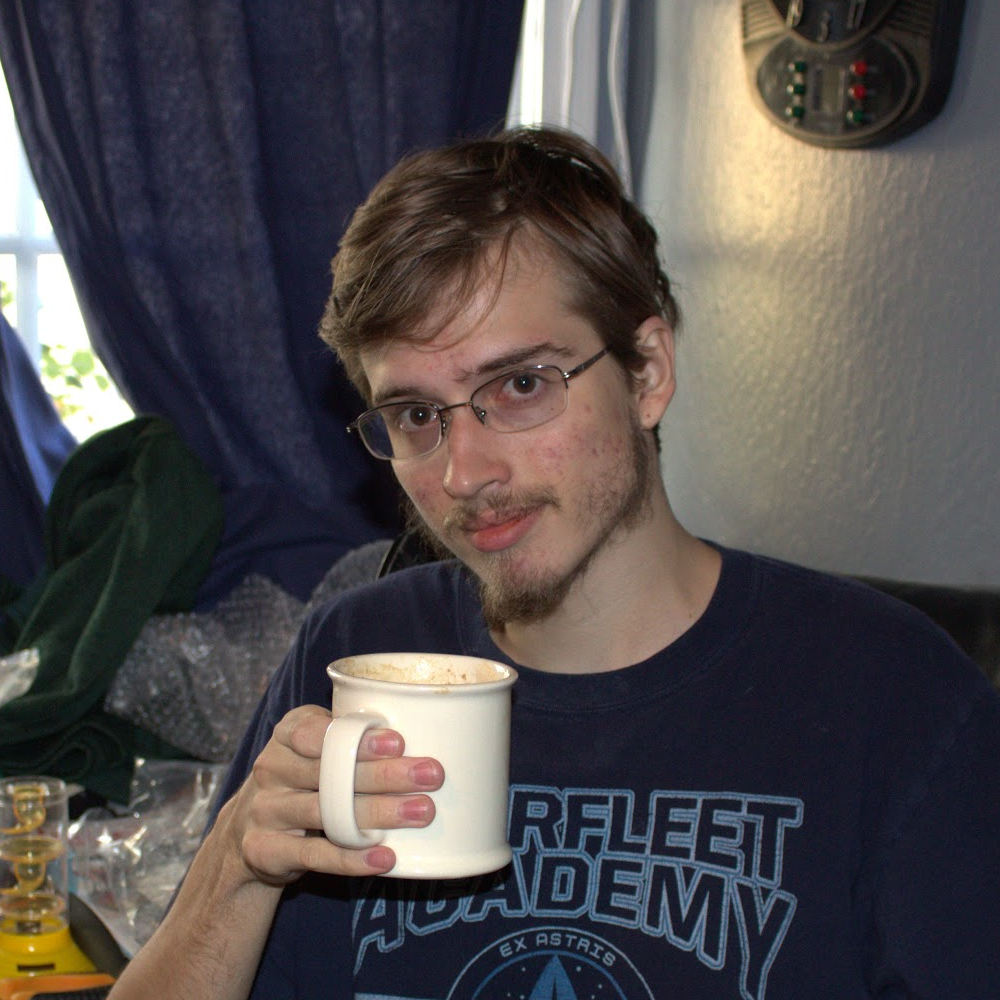
\includegraphics[width=1.5in]{MelCoffeeCropped.jpg}
	
	\vspace*{0.25in}
	
	\parbox{1.75in}{
		
		\color{white}\large Mel McCalla \normalsize is a high school senion attending Palo Alto Preparatory High
		School.  A lover of books, coffee and sci-fi, he regularly enjoys his coffee and Star Trek.  He will be
		attending University of Oregon in the fall, where he plans to study Pure Mathematics and Computer Science. }
	
}

\end{bookcover}

\end{document} 